You can find the code and everything else also on GitHub under the link \textit{https://github.com/awilsee/CSec}. Maybe more convenient for you.


\section{Implement Diffie Hellman Key Exchange}
\lstinputlisting[caption=Code of task 1, label=lst:task1]{task1.py}

\textit{How hard would it be for an adversary to solve the Diffie Hellman Problem (DHP) given these parameters? What strategy might the adversary take?}\\
With p = 37 and g = 5 it could be relatively easy to guess respectively to calculate these numbers. Because these two numbers have to be primes and the adversary also knows the algortihm behind it, so  he can try out some numbers. Because they are very small with only some bits it's possible in a resonable time.\\

\textit{Would the same strategy used for the tiny parameters work here? Why or why not?}\\
No, it wouldn't because the prime numbers are now to large, so there are two many possibilities to calculate, it would take several years to get the right numbers.\\

\section{Implement MITM Key Fixing \& Negotiated Groups}
\lstinputlisting[caption=Code of task 2, label=lst:task2]{task2.py}

\textit{Why were these attacks possible? What is necessary to prevent them?}\\
All these attacks works in the same way, because with to calculate the modulo of a multiple of the same number results in 0 or in the other examples 1. So the private secret key doesn't really come into effect. \\
One way to prevent this would be a check if g is a p, 0 or 1. or the results afterwards.\\


\section{Implement textbook RSA \& MITM Key Fixing via Malleability}
\lstinputlisting[caption=Code of task 3, label=lst:task3]{task3.py}
\lstinputlisting[caption=Code of task 3 - PrimesRabinMiller, label=lst:PrimesRabinMiller]{PrimesRabinMiller.py}

\subsection{A}
\textit{While it's very common for many people to share an e (common values are 3,7, 2\textsuperscript{16}+1), it is very bad if two people share an RSA modulus n. Briefly describe why this is, and what the ramifications are.}\\
It is common for e because it simplifies the encryption and doesn't take too long for encryption for example if you use 2\textsuperscript{16}+1 there are only two bits 1. n shouldn't be shared because then you take the same both prime numbers. If you have different msg from different people with the same key you can start guessing and get the key more easily.\\

\subsection{B}
\textit{Give another example of how RSA’s malleability could be used to exploit a system (e.g. to cause confusion, disruption, or violate integrity).}\\
In the listing \ref{lst:task3} starting at line 118 the example of malleability is that Mallory change c' to n which results in 0 for s as explained earlier.\\
Another example would be if you think on an auction where anybody send their encrypted bits. Mallory can multiply the bid from someone else even without encryption and knowing how much the other bid.\\

\textit{Suppose Mallory sees the signatures for two message m1 and m2.  Show how Mallory can create a valid signature for a third message, m3 = m1 * m2.}\\
If the message is signed, Mallory can use the same attack to get to the messages as well as write some messages.\\

\subsection{C}
\textit{Briefly justify whether either of the following key exchange protocols do or do not provide forward secrecy.}\\
Well, neither protocol prevents brute-force attacks on the underlying ciphers, however with such a session key you prevent that your communications from the past can't be read by compromising your private key. It is mostly combined with the Diffie Hellman or even better with Elliptic Curve Diffie Hellman.\\
If an attacker can get the private key of the server the RSA isn't secure anymore because the session key correspond with the keys and therefore all sessions can be decrypted.\\
However you can use Perfect Forward Secrecy in this case which removes the link between servers and sessions key.


\section{Performance of RSA and AES}

\begin{figure}[htp]
    \centering
    \caption{AES}
    \label{fig:aes}
    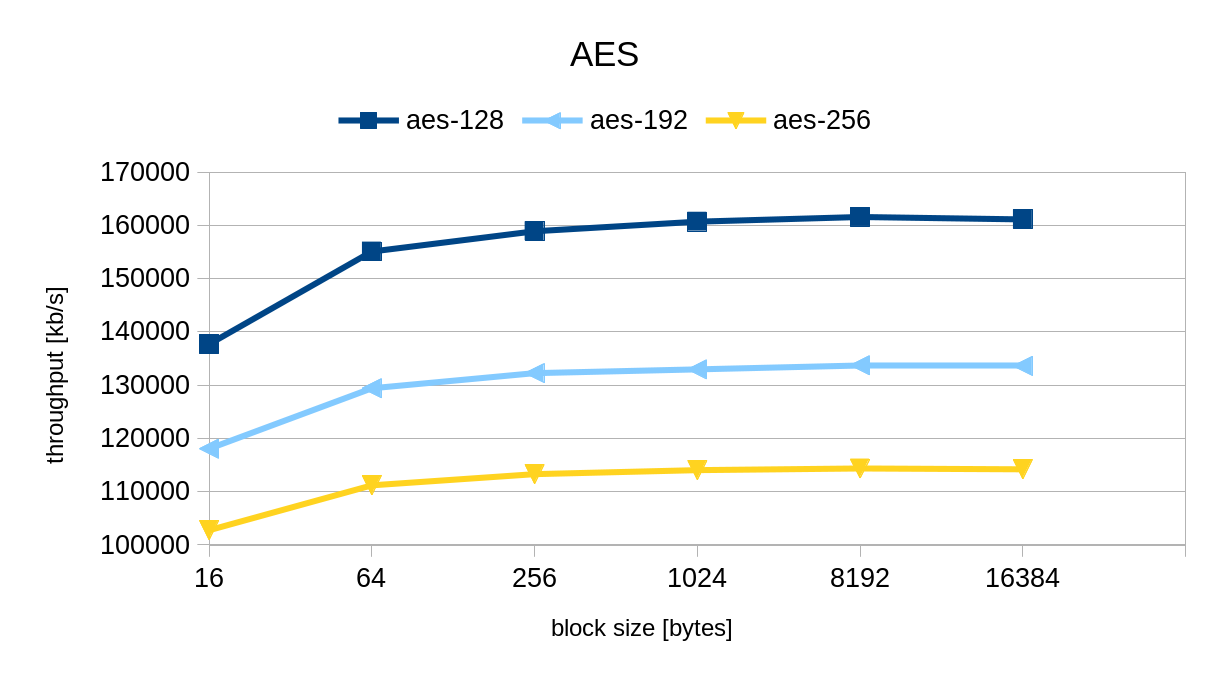
\includegraphics[width=\textwidth]{aes.png}
\end{figure}

On figure \ref{fig:aes} you can see that the larger the keys sizes the slower it gets. Whereas the throughout gets higher the larger the block size is.

\begin{figure}[htp]
    \centering
    \caption{RSA}
    \label{fig:rsa}
    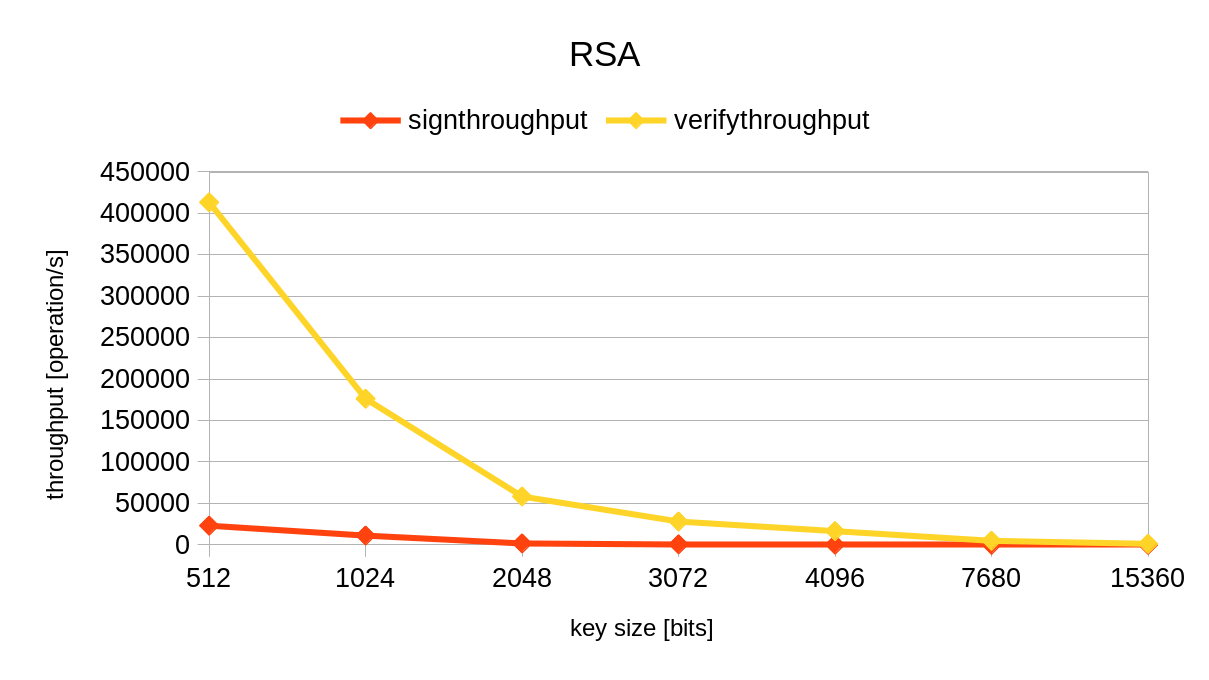
\includegraphics[width=\textwidth]{rsa.png}
\end{figure}
On figure \ref{fig:rsa} you can see that throughput is decreasing the larger the key size gets. Additionally the verification operation is significantly faster than signing.\\
Though it's hard to compare them in detail, because the speed for RSA is measured in operations whereas the speed for AES is measured in kbit/s so its two different methods. Furthermore block size and key size is also not the same. Conspicuous is that at AES the throughput is increasing with the larger block size and at RSA it's decreasing.